\documentclass[a4paper,12pt,oneside]{book}

%-------------------------------Start of the Preable------------------------------------------------
\usepackage[english]{babel}
\usepackage{blindtext}
\usepackage{float}
%packagr for hyperlinks
\usepackage{hyperref}
\hypersetup{
    colorlinks=true,
    linkcolor=blue,
    filecolor=magenta,      
    urlcolor=cyan,
}

\urlstyle{same}
%use of package fancy header
\usepackage{fancyhdr}
\setlength\headheight{26pt}
\fancyhf{}
%\rhead{
\includegraphics[width=1cm]{logo}}
\lhead{\rightmark}
\rhead{
\includegraphics[width=1cm]{logo}}
\fancyfoot[RE, RO]{\thepage}
\fancyfoot[CE, CO]{\href{http://www.e-yantra.org}{www.e-yantra.org}}

\pagestyle{fancy}

%use of package for section title formatting
\usepackage{titlesec}
\titleformat{\chapter}
  {\Large\bfseries} % format
  {}                % label
  {0pt}             % sep
  {\huge}           % before-code
 
%use of package tcolorbox for colorful textbox
\usepackage[most]{tcolorbox}
\tcbset{colback=cyan!5!white,colframe=cyan!75!black,halign title = flush center}

\newtcolorbox{mybox}[1]{colback=cyan!5!white,
colframe=cyan!75!black,fonttitle=\bfseries,
title=\textbf{\Large{#1}}}

%use of package marginnote for notes in margin
\usepackage{marginnote}

%use of packgage watermark for pages
%\usepackage{draftwatermark}
%\SetWatermarkText{
\includegraphics{logo}}
\usepackage[scale=2,opacity=0.1,angle=0]{background}
\backgroundsetup{
contents={
\includegraphics{logo}}
}

%use of newcommand for keywords color
\usepackage{xcolor}
\newcommand{\keyword}[1]{\textcolor{red}{\textbf{#1}}}

%package for inserting pictures
\usepackage{graphicx}

%package for highlighting
\usepackage{color,soul}

%new command for table
\newcommand{\head}[1]{\textnormal{\textbf{#1}}}


%----------------------End of the Preamble---------------------------------------


\begin{document}

%---------------------Title Page------------------------------------------------
\begin{titlepage}
\raggedright
{\Large eYSIP2016\\[1cm]}
{\Huge\scshape Raspberry Pi Hardware Development \& Tutorials \\[.1in]}
\vfill
\begin{flushright}
{\large Aditya Kumar \\}
{\large Pritish Salunke \\}
{\large Rutuja Ekatpure \\}
{\large Deepa Avudiappan \\}
{\large Duration of Internship: $ 21/05/2016-10/07/2016 $ \\}
\end{flushright}

{\itshape 2016, e-Yantra Publication}
\end{titlepage}
%-------------------------------------------------------------------------------

\chapter[Project Tag]{Raspberry Pi Hardware Development \& Tutorials}
\section*{Abstract}
Interfacing LED, switch, LCD and ICs on Raspberry Pi. Create a module of each device interfaced. Communication between Raspberry Pi and other device using Zigbee and Bluetooth module.Communication between Raspberry Pi and Firebird V using SPI, I2C and UART protocol. Create documentation and video tutorial explaining individual module. Design PCB for the devices interfaced with Raspberry Pi.

\subsection*{Completion status}
\begin{itemize}
    \item \textbf{Task 1:}  \\ 
            Developed different modules for Raspberry Pi \\
            E.g. PWM Driver IC PCA9685, ADC, Port Expander etc. \\
    \item \textbf{Task 2:} \\
            Communication between Rpi and other \\
            device through Xbee and Bluetooth Module \\
    \item \textbf{Task 3:} \\
            Interfacing LCD with Raspberry Pi  \\
    \item \textbf{Task 4:}  \\
            Communication between Raspberry Pi and \\
            Firebird V using UART protocol    \\
    \item \textbf{Task 5:}  \\
            Communication between Raspberry Pi  
            and Arduino UNO       
            using I2C and SPI protocol     \\
    \item \textbf{Task 6:} \\
            Designed PCBs for \\
            \begin{enumerate}
            \item LCD connected with port expander IC MCP23017 IC
            \item LM35 temperature sensor and Sharp IR sensor with ADC IC MCP3008
            \item PWM driver IC PCA9685 to drive DC motor and Servo motor 
            \item Xbee and Bluetooth module 
            \end{enumerate}
              
\end{itemize}
    


\section{Hardware parts}
\begin{itemize}
  \item List of hardware 
  \begin{enumerate}
      \item Raspberry Pi \\
      \href{https://cdn-shop.adafruit.com/pdfs/raspberrypi2modelb.pdf} {Download link}
      \href{http://www.amazon.in/Raspberry-Pi-Model-1GB-Complete/dp/B00T2U7R7I} {Vendor Link}
      \item FireBird V Robot \\
      \href{http://www.atmel.com/Images/Atmel-2549-8-bit-AVR-Microcontroller-ATmega640-1280-1281-2560-2561_datasheet.pdf} {Download link}
      \href{http://www.nex-robotics.com/products/fire-bird-v-robots/fire-bird-v-atmega2560-robotic-research-platform.html} {Vendor Link}
      \item LED
      \item Resistor
      \item Switch
      \item LCD   \\
      \href{http://www.agspecinfo.com/pdfs/J/JHD162A.PDF} {Download link}
      \href{http://www.amazon.in/JCE-16x2-LCD-Display/dp/B00OVY28M4} {Vendor Link}
      \item MCP23017 IC     \\
      \href{https://cdn-shop.adafruit.com/datasheets/mcp23017.pdf} {Download link}
      \href{http://www.smddevices.com/} {Vendor Link}
      \item MCP3008 IC       \\
      \href{https://cdn-shop.adafruit.com/datasheets/MCP3008.pdf} {Download link}
      \href{http://www.dnatechindia.com/MCP3008-10-Bit-ADC.html} {Vendor Link}
      \item Sharp Sensor      \\
      \href{http://www.sharpsma.com/webfm_send/1208} {Download link}
      \href{http: //www.ebay.in/itm/262401450416?aff_source=Sok-Goog} {Vendor Link}
      \item LM35 Temperature Sensor    \\
      \href{http://www.ti.com/lit/ds/symlink/lm35.pdf} {Download link}
      \href{http://www.amazon.in/Robo-India-Temperature-Sensor-LM35/dp/B00WO5AFPE} {Vendor Link}
      \item PCA9685 PWM Driver IC  \\
      \href{https://cdn-shop.adafruit.com/datasheets/PCA9685.pdf} {Download link}
      \href{http://www.amazon.in/Channel-Servo-Motor-Driver-Controller-PCA9685/dp/B01D4I8KII?tag=googinhydr18418-21&tag=googinkenshoo-21&ascsubtag=a4459339-54b9-4883-ac3e-2de2611b95a1} {Vendor Link}
      \item L293D Motor Driver IC       \\
      \href{http://www.ti.com/lit/ds/symlink/l293.pdf} {Download link}
      \href{http://www.amazon.in/L293D-Push-Pull-Four-Channel-Stepper-Driver/dp/B00MYZPL4Y?tag=googinhydr18418-21&tag=googinkenshoo-21&ascsubtag=a4459339-54b9-4883-ac3e-2de2611b95a1} {Vendor Link}
      \item Capacitor
      \item DC Motor
      \item Servo Motor
      \item 9 V battery
      \item Xbee Module  \\
      \href{https://www.sparkfun.com/datasheets/Wireless/Zigbee/XBee-Datasheet.pdf} {Download link}
      \href{http://www.amazon.in/XBee-2mW-Wire-Antenna-ZigBee/dp/B007R9U1QA?tag=googinhydr18418-21&tag=googinkenshoo-21&ascsubtag=a4459339-54b9-4883-ac3e-2de2611b95a1} {Vendor Link}
      \item Bluetooth Module      \\
      \href{http://www.linotux.ch/arduino/HC-0305_serial_module_AT_commamd_set_201104_revised.pdf} {Download link}
      \href{http://www.amazon.in/Verve-VTA009-Bluetooth-Module-HC-05/dp/B00S15XTG8?tag=googinhydr18418-21&tag=googinkenshoo-21&ascsubtag=a4459339-54b9-4883-ac3e-2de2611b95a1} {Vendor Link}
      \item Arduino UNO   \\
      \href{http://www.mouser.com/pdfdocs/Gravitech_ATMEGA328_datasheet.pdf} {Download link}
      \href{http://www.amazon.in/Arduino-UNO-board-DIP-ATmega328P/dp/B008GRTSV6} {Vendor Link}
  \end{enumerate}
\end{itemize}

\section{Software used}
\begin{itemize}
  \item List of software used 
  \begin{enumerate}
      \item MobaXterm Personal Edition \\
      \href{http://mobaxterm.mobatek.net/MobaXterm_Setup_9.1.msi} {Download link}
      \item Raspbian Jessie   \\
      \href{https://downloads.raspberrypi.org/raspbian_latest}{Download Link}
      \item Atmel Studio 6.0 \\
      \href{http://atmel-studio.software.informer.com/download/?ca56297}{Download Link}
      \item Eagle Version 7.6.0 \\
      \href{http://www.cadsoftusa.com/download-eagle/}{Download Link}
      \item NEX ISP USB STK500V2 Programmer \\
      \href{http://www.nex-robotics.com/images/downloads/NEX\%20AVR\%20STK500V2.zip}{Download Link}
      \item XCTU \\
      \href{http://www.digi.com/products/xbee-rf-solutions/xctu-software/xctu#productsupport-utilities}{Download Link}
      \item Arduino 1.6.9  \\
       \href{https://www.arduino.cc/en/Main/Software}{Download Link}
      \item Camtasia Studio 8 \\
      \href{http://filehippo.com/download_camtasia_studio/download/fc20113e4355b8a0434494faa4ca14e3/}{Download Link}
      
      
  \end{enumerate}
\end{itemize}

\section{Accessing GPIO pins of Raspberry Pi}
\flushleft
In this experiment we have interfaced an led and switch. Resistor is connected with led to limit the current. \\
\textbf{Problem Statement} \\
When switch is pressed led will turn on. Again when switch is pressed led will turn off.\\
\textbf{Circuit Diagram}\\
\begin{figure}[H]
    \centering
    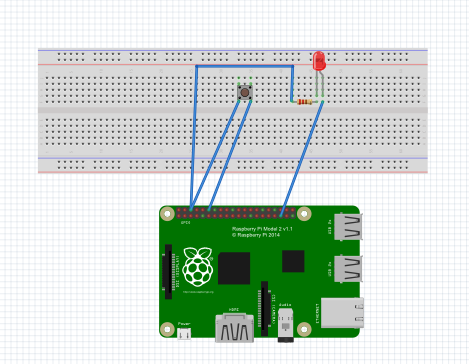
\includegraphics[scale=0.6]{GPIO}
    \caption{}
\end{figure}
\subsection*{Assembly of hardware}
\subsection*{Step 1}
One pin of the push button is connected to Ground(Pin 9).
\subsection*{Step 2}
The other pin of the push button is connected to IC pin no. 12.
\subsection*{Step 3}
The anode of led is connected to IC pin 35 of raspberry pi.
\subsection*{Step 4}
The cathode of led is connected to the the resistor of 300 ohms which
is then connected to the ground.

\section{Enabling I2C interface in Raspberry Pi}
I2C stands for Inter Integrated Circuit. It is a communication protocol in which many devices are connected with two signal line SDA(Serial Data) and Serial Clock(SCL).
Since I2c interface is disabled by default. So, in following steps we have explained how to enable I2C interface on RPi. 
\textbf{Steps to enable I2C interface on RPi}
\begin{enumerate}
		\item Open MobaXterm. 
		\item Establish SSH connection to R-Pi.
		\item Under Advanced SSH settings.
		\subitem If in remote environment you have chosen Interactive shell.
		\subitem If in remote environment you have chosen LXDE desktop then open LXTerminal.
		
		\item  Type \textit{sudo raspi-config}. This will launch the raspi-config utility.
		
		\begin{figure}[h!]
			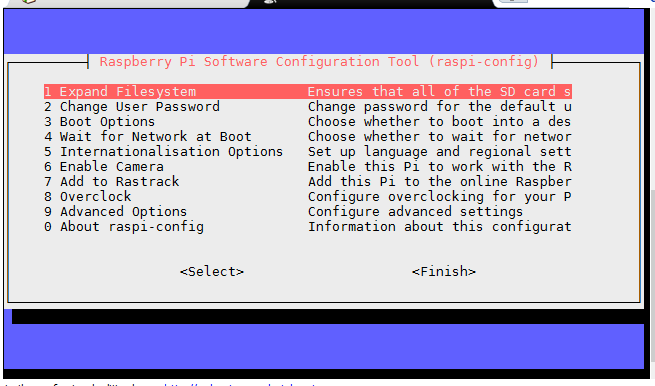
\includegraphics[width=11cm,height=5cm]{i2c_1}
			\centering
			\caption{[4]}
			\end{figure}
		\item Select the \textit{Advanced options}
		\begin{figure}[h!]
			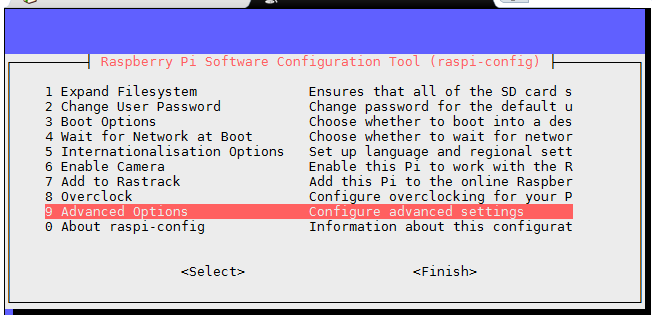
\includegraphics[scale=0.6]{i2c_2}
			\centering
			\caption{[4]}
		\end{figure} 
		\item Then select \textit{option A7 I2C} 
		\newline
		\begin{figure}[h!]
			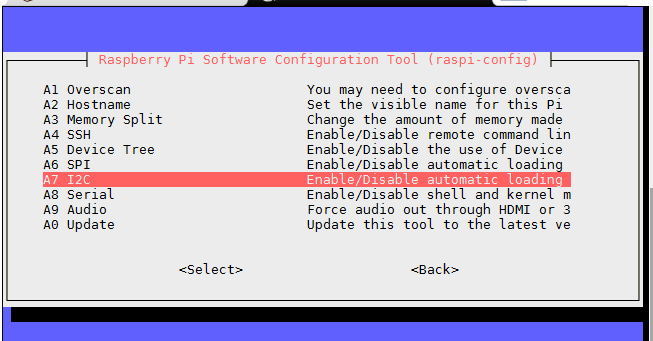
\includegraphics[scale=0.6]{i2c_3}
			\centering
			\caption{[4]}
		\end{figure}
		\item It will ask to enable the ARM I2C interface, click \textit{YES}.
		\newline
		\begin{figure}[h!]
			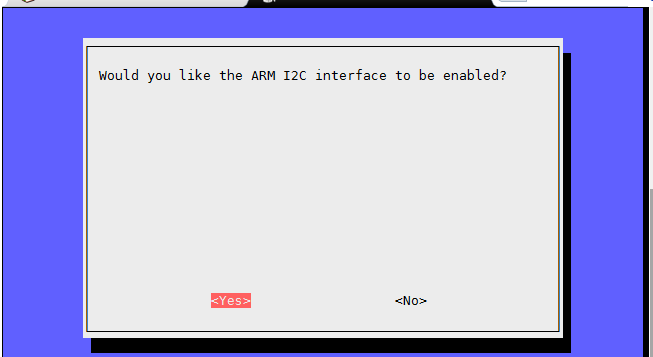
\includegraphics[scale=0.6]{i2c_4}
			\centering
			\caption{[4]}
		\end{figure}
		\newpage
		\item Then it will ask if you would like I2C kernel module to be uploaded by default. Select\textit{YES}.
		\begin{figure}[h!]
			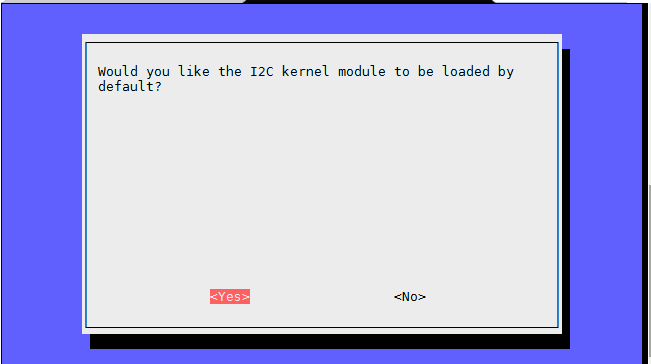
\includegraphics[scale=0.6]{i2c_5}
			\centering
			\caption{[4]}
		\end{figure}
		\item I2C kernel module will now be loaded by default.Click \textit{OK}
		\begin{figure}[h!]
			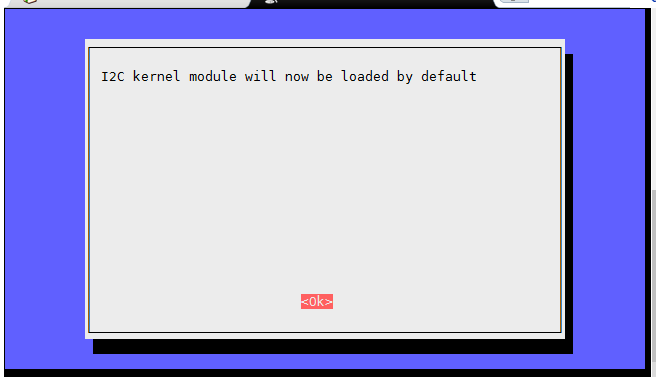
\includegraphics[scale=0.6]{i2c_6}
			\centering
			\caption{[4]}
		\end{figure}
		\item Select Finish to return to command line.
		\item Next we need to edit the modules file using : \newline \textit{sudo nano /etc/modules} 
		\begin{figure}[h!]
			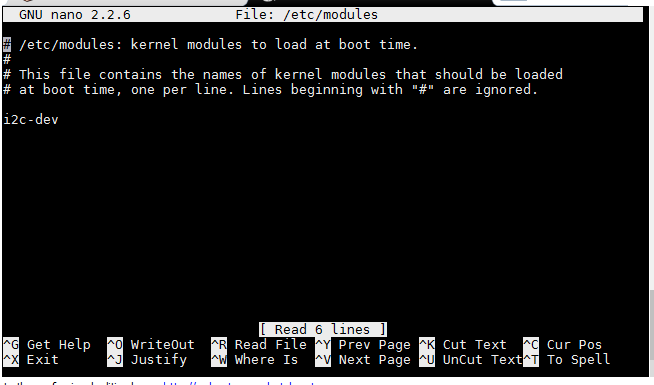
\includegraphics[scale=0.6]{i2c_7}
			\centering
			\caption{[4]}
		\end{figure}
		\newpage
		\item Add the following two lines : \newline \textit{i2c-bcm2708 \newline i2c-dev}
		
		\begin{figure}[h!]
			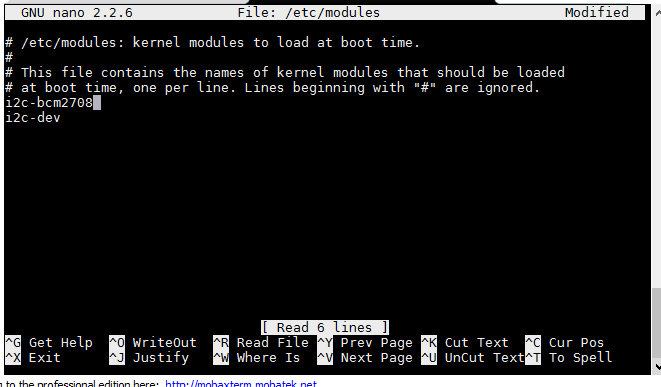
\includegraphics[scale=0.6]{i2c_8}
			\centering
			\caption{[4]}
		\end{figure}
		\item Use CTRL-X, then Y, then RETURN to save the file and exit.
		\item To help debugging and allow the i2c interface to be used within Python we can install “python-smbus” and “i2c-tools” : \newline \textit{sudo apt-get update \newline sudo apt-get install -y python-smbus i2c-tools}
		\item Shutdown your Pi using : \newline \textit{sudo halt} \newline Wait ten seconds, disconnect the power to your Pi and you are now ready to connect your I2C hardware.
		\item When you power up or reboot your Pi you can check the i2c module is running by using the following command : \newline \textit{lsmod | grep i2c\_} \newline That will list all the modules starting with “i2c\_”. If it lists “i2c\_bcm2708” then the module is running correctly.
		\item Once you have connected your hardware double check the wiring. Make sure 3.3V is going to the correct pins and you have got not short circuits. Power up the Pi and wait for it to boot.
		\item Type the command: \newline \textit{sudo i2cdetect -y 1} 
		\item You should the output as:
			\begin{figure}[h!]
				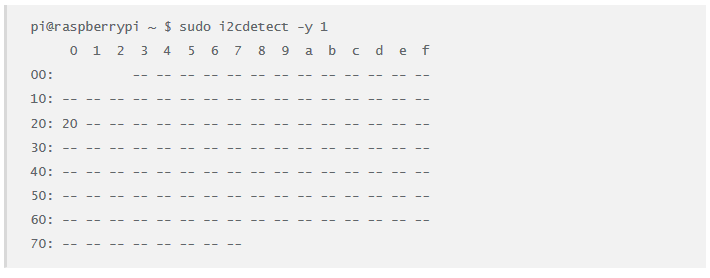
\includegraphics[scale=0.6]{i2c_9}
				\centering
				\caption{[4]}
			\end{figure}	
	\end{enumerate}
\newpage

\section{Interfacing Port Expander MCP23017 IC}
In this experiment we have interfaced port expander MCP23017 IC with RPi. Port expander is used to increase GPIO pins of RPi.  \\
\textbf{Problem Statement}
Interface an LCD with port expander MCP23017 IC and display some message.\\
\textbf{Circuit Diagram}\\
\begin{figure}[H]
    \centering
    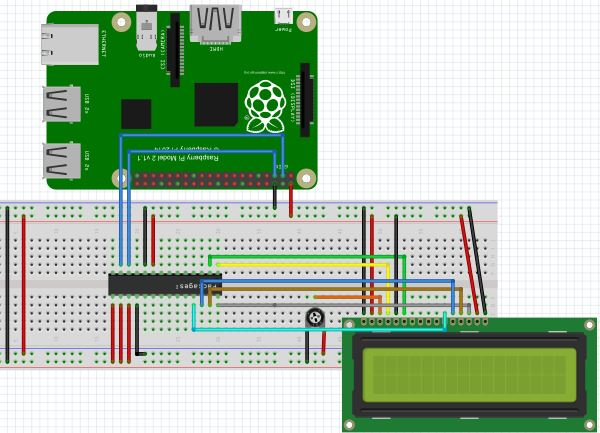
\includegraphics[scale=0.4]{port_expander_lcd}
    \caption{LCD connected to MCP23017 IC}
\end{figure}
\newpage
\textbf{Schematic Diagram}\\
\begin{figure}[H]
    \centering
    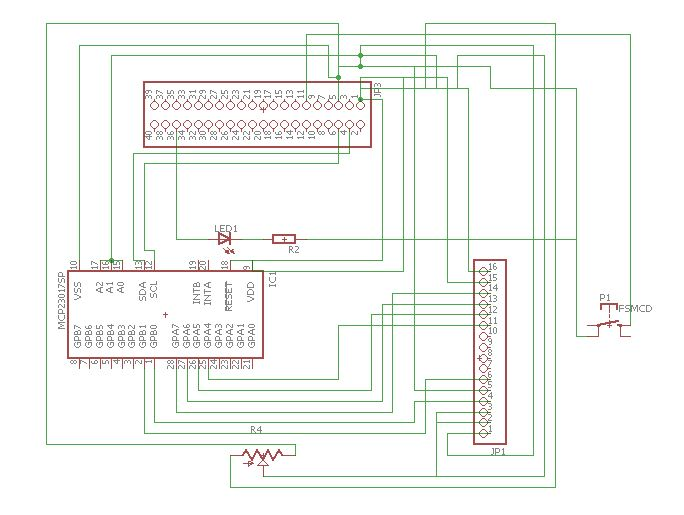
\includegraphics[scale= 0.8]{LCD_schematic}
    \caption{Eagle Schematic}
\end{figure}
\textbf{PCB Layout}\\
\begin{figure}[H]
    \centering
    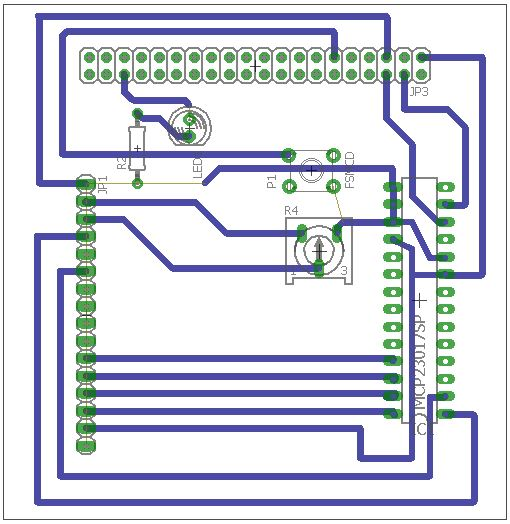
\includegraphics[scale= 0.4]{lcd_pcb_layout}
    \caption{PCB Layout}
\end{figure}
\subsection*{Assembly of hardware}
\subsection*{Step 1}
Pin 9 (VDD) is connected to 5V
\subsection*{Step 2}
Pin 10 (VSS) is connected to Ground
\subsection*{Step 3}
Pin 12 (SCL) is connected to Pin 5 on the Pi GPIO
\subsection*{Step 4}
Pin 13 (SDA) is connected to Pin 3 on the Pi GPIO
\subsection*{Step 5}
Pin 18 (Reset) should be set high for normal operation so we connect this to 5V
\subsection*{Step 6}
Pins 15, 16 \& 17 (A0-A2) determine the number assigned to this device. We are only using one device so we will give it a binary zero by setting all three of these pins to 0 (ground)
\subsection*{Step 7}
RS and Enable pins of the LCD are connected to GPB0 and GPB1 respectively.
\subsection*{Step 8}
R/W pin is Grounded
\subsection*{Step 9}
Data pins D7,D6,D5 and D4 are connected to GPA7,GPA6,GPA5 and GPA4 respectively.

\section{Interfacing ADC IC MCP3008}
\textbf{Description:} \\
Raspberry Pi does not have internal ADC. So,to read the values of analog sensors 
we need to provide external ADC. Here, we will be using MCP3008 IC. 
The MCP3008 is a successive approximation 10bit 8-channel Analogue-to-digital 
converter (ADC). It is cheap, easy to connect and doesnt require any additional 
components.It uses the SPI bus protocol which is supported by the Pis GPIO 
header.\\
\textbf{Problem Statement:}
Read the values of LM35 temperature sensor by using MCP3008 IC(ADC) and calibrate
it by programming in python.
\textbf{Circuit Diagram}\\
\centering 
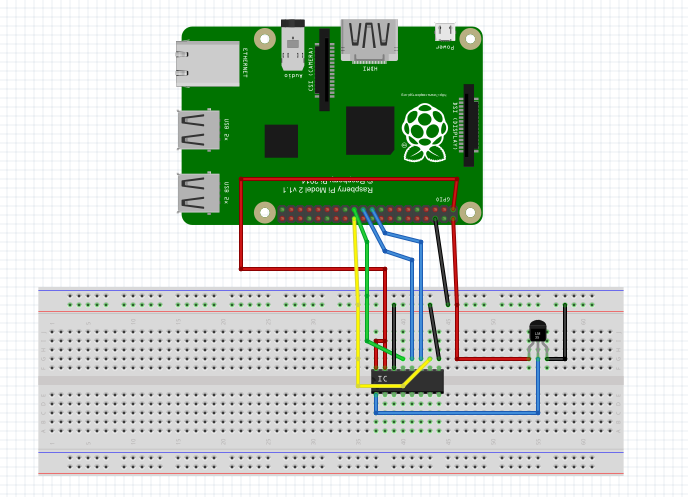
\includegraphics[scale=0.4]{lm35_interfacing}
\flushleft
\textbf{Schematic Diagram}\\
\centering
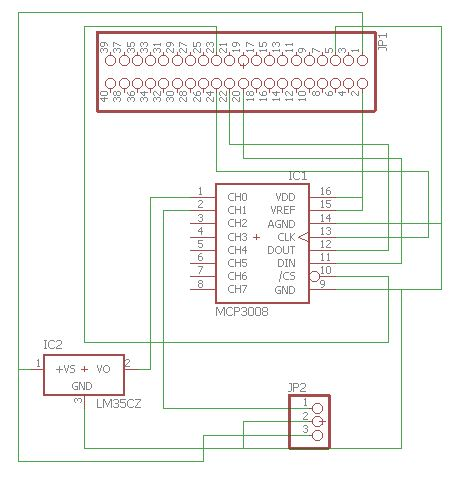
\includegraphics[scale=0.4]{adc_schematic}
\flushleft
\textbf{PCB Layout}\\
\centering
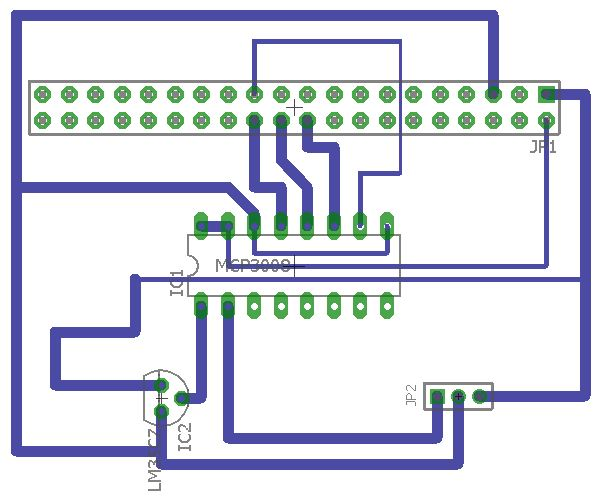
\includegraphics[scale=0.4]{adc_layout}
\flushleft
Fig. shows PCB Layout

\section{Interfacing DC Motor}
\textbf{Description:} \\
Normal DC gear-head motors require current greater than 250mA. Most of
the ICs like 555 timer,74 series ICs cannot supply this amount of
current.Instead if we directly connect motors to the output of any of the
above IC's, they might get damaged. There is a need of a circuitry that
can act as a bridge between the above mentioned ICs and the motors. This
is where a motor driver plays a crucial role. It regulates the current owing through the circuit hence preventing any damage to the device.
L293D is dual H-bridge motor driver ICs. Using these we can control the
rotation of two motors in both clockwise and anti-clockwise direction. \\
\textbf{Problem Statement:} \\
Controlling the speed of DC motor by using Port expander IC MCP23017 and motor
driver IC L293D. \\
\textbf{Circuit Diagram}\\
\centering
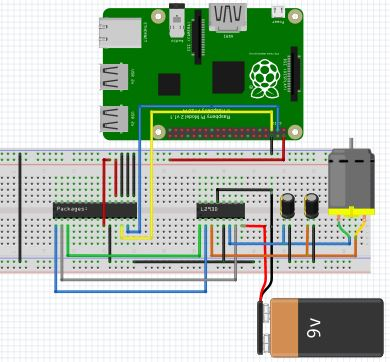
\includegraphics[scale=0.6]{dc_motor_I2C}
\flushleft
Fig. shows the conncection diagram.
\subsection*{Assembly of hardware}
\subsection*{Step 1}
Pin 9 (VDD) is connected to 5V
\subsection*{Step 2}
Pin 10 (VSS) is connected to Ground
\subsection*{Step 3}
Pin 12 (SCL) is connected to Pin 5 on the Pi GPIO
\subsection*{Step 4}
Pin 13 (SDA) is connected to Pin 3 on the Pi GPIO
\subsection*{Step 5}
Pin 18 (Reset) should be set high for normal operation so we connect
this to 5V
\subsection*{Step 6}
Pins 15, 16 \& 17 (A0-A2) determine the number assigned to this device. We are only using one device so we will give it a binary zero by setting all three of these pins to 0 (ground)
\subsection*{Step 7}
Input 1 and Input 2 of L293D is connected to GPB0 and GPB1 of MCP23017
\subsection*{Step 8}
Pin 1 (enable pin) of L293D is connected to GPB2.
\subsection*{Step 9}
Out 1 and Out 2 are connected to a DC motor.
\section{Interfacing Servo motor using PWM Driver IC PCA9685}
\textbf{Description:} \\
Raspberry Pi has only one pin for PWM generation, which is pin number 12. So, if 
we want to control the speed of more than one motor by changing its PWM then we 
need PCA9685 motor driver IC.
PCA9685 is an I2C-bus controlled 16-channel PWM Driver IC.Each PWM channel output 
has its own 12-bit resolution (4096 steps) fixed frequency individual PWM 
controller that operates at a programmable frequency from a typical of 24 Hz 
to 1526 Hz with a duty cycle that is adjustable from 0% to 100% to allow the motor
to be set to a specific PWM value. All outputs are set to the same PWM frequency.\\
\textbf{Problem Statement:} \\
Controlling the angle or duty ratio of servo motor using PCA9685 PWM Driver IC.
\newpage
\textbf{Circuit Diagram}\\
\centering 
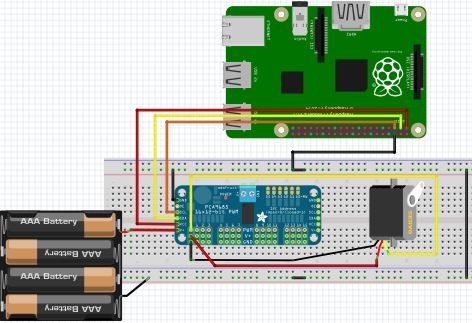
\includegraphics[scale=0.6]{servo_motor_PCA9685}
\flushleft
Fig. above shows connections.
\subsection*{Assembly of hardware}
\subsection*{Step 1}
Control pin of servo motor is connected to S pin of channel 0.
\subsection*{Step 2}
Ground and Vcc of servo motor is connected to ground and Vcc of channel 0 of PCA9685 respectively. 
\subsection*{Step 3}
Pin 12 (SCL) is connected to Pin 5 on the RPi GPIO
\subsection*{Step 4}
Pin 13 (SDA) is connected to Pin 3 on the RPi GPIO
\subsection*{Step 5}
Vcc of IC is connected to pin 2 on the RPi.
\subsection*{Step 6}
Ground pin of IC is connected to pin 6 of RPi.
\subsection*{Step 7}
V+ of IC is connected positive terminal of 9V battery.

\section{Serial Communication using Xbee and Bluetooth Module}
\textbf{Circuit Diagram of Bluetooth and Raspberry Pi}  \\
\centering
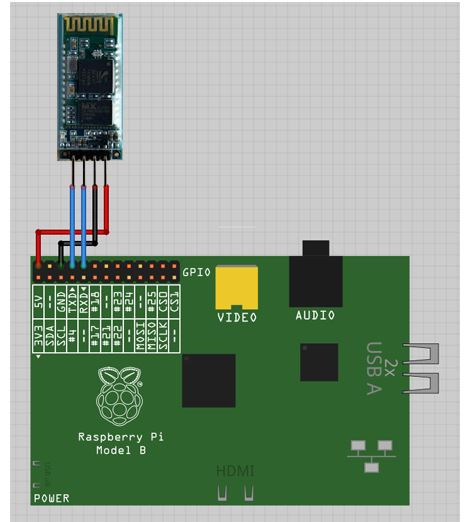
\includegraphics[scale = 0.6]{bluetooth}
\flushleft
Fig. shows Connection Diagram.
\subsection*{Assembly of harware}
\subsection*{Step 1}
Pin 2 of RPi is connected to Vcc.
\subsection*{Step 2}
Pin 6 of Rpi is connected to ground.
\subsection*{Step 3}
Pin 8(TXD) of RPi is connected to RXD pin.
\subsection*{Step 4}
Pin 10 (RXD) is connected to TXD pin of bluetooth module.
\subsection*{Connection Diagram of Xbee and Raspberry Pi}
\centering
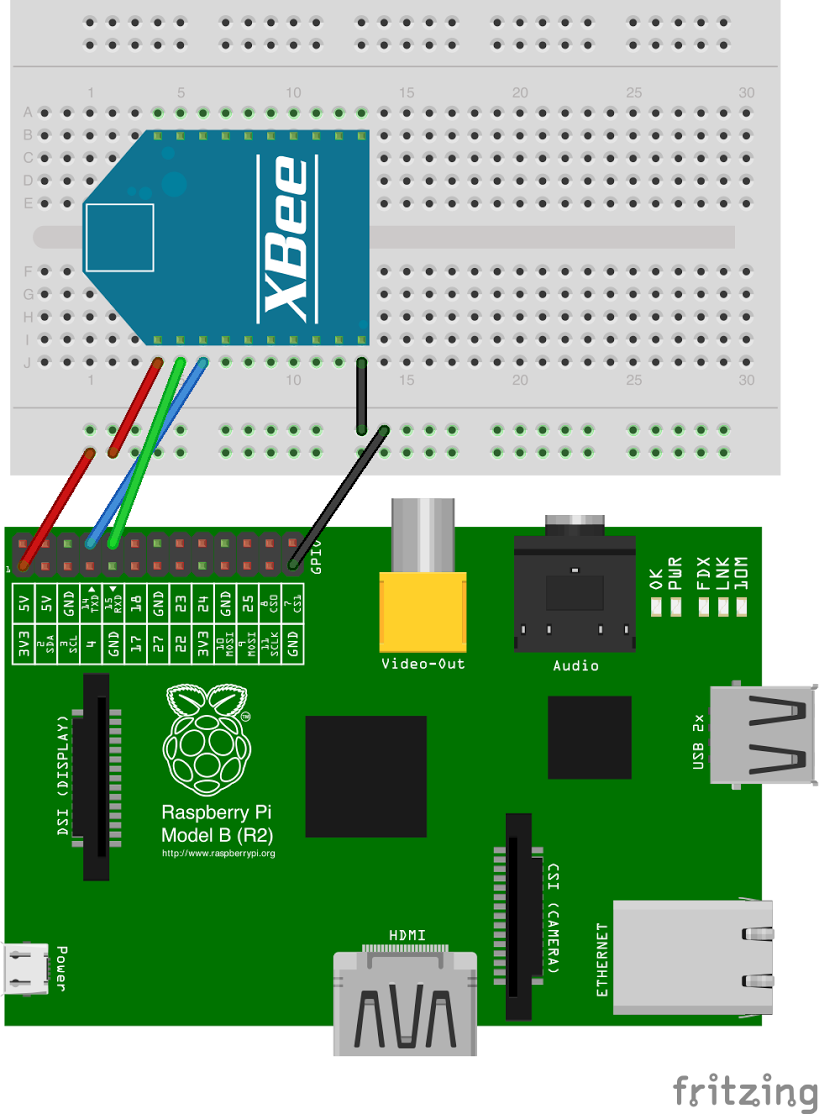
\includegraphics[scale=0.2]{raspi_to_xbee}
\flushleft
Fig. shows connection diagram.
\subsection*{Assembly of harware}
\subsection*{Step 1}
Connect Vcc to pin 2 (5V) of Rpi.
\subsection*{Step 2}
Ground is connected to pin 6 (GND) of RPi.
\subsection*{Step 3}
Pin TXD of Xbee is connected to pin 10 (RXD) of RPi.
\subsection*{Step 4}
Pin RXD of Xbee is connected to pin 8 (TXD) of RPi.
\textbf{Schematic Diagram of Bluetooth and Xbee Module}\\
\centering
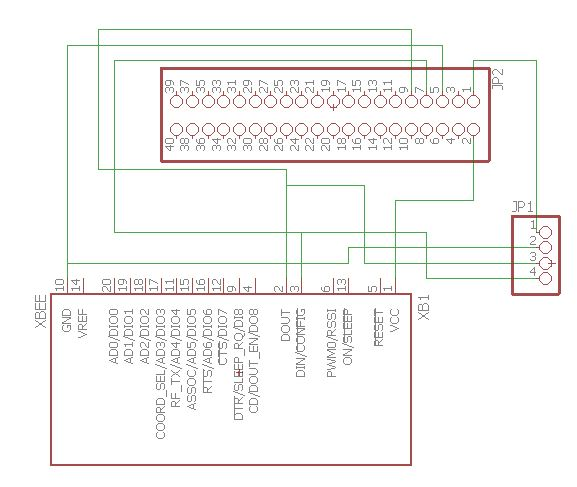
\includegraphics[scale= 0.8]{zigbee_schematic}
\flushleft
\textbf{PCB Layout}\\
\centering
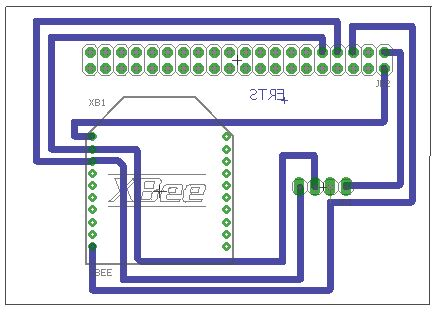
\includegraphics[scale= 0.5]{zigbee_layout}
\flushleft
Above figure shows our PCB Layout.
\section{Interrupt on Raspberry Pi}
\subsection*{External Interrupt on RPi}

\textbf{Circuit Diagram}  \\
\centering
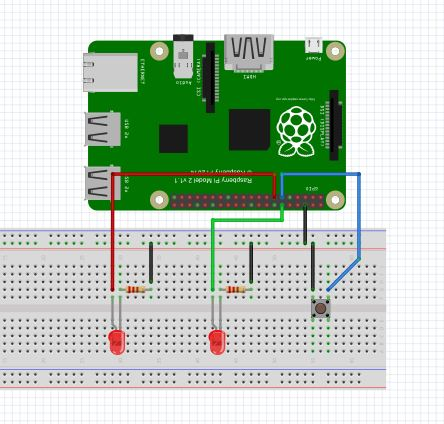
\includegraphics[scale = 0.6]{switch_interrupt}
\flushleft
Fig. shows Connection Diagram.
\subsection*{Assembly of harware}
\subsection*{Step 1}
Pin 11 is connected to switch and other terminal of switch is grounded.
\subsection*{Step 2}
Pin 12 of Rpi is connected to anode of one of the LED. Cathode of LED is connected to ground through a current limiting resistor.
\subsection*{Step 3}
Pin 13 of Rpi is connected to anode of second LED. Cathode of second LED is connected to ground through a current limiting resistor.


\subsection*{Interrupt on Raspberry Pi using SPI protocol}
\textbf{Circuit Diagram}  \\
\centering
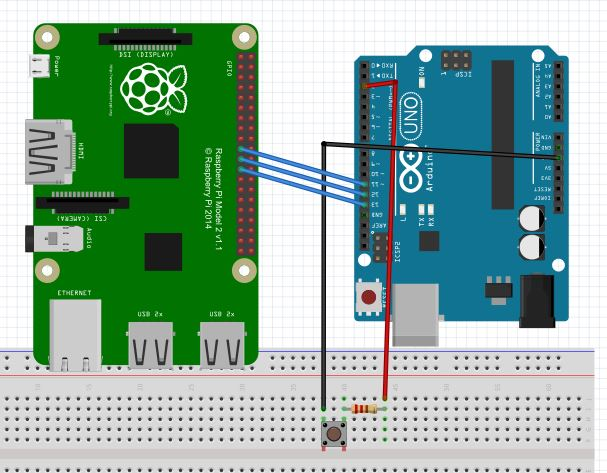
\includegraphics[scale = 0.6]{rpi_with_arduino_spi}
\flushleft
Fig. shows Connection Diagram.
\subsection*{Assembly of harware}
\subsection*{Step 1}
Pin 11 of arduino is connected to MOSI(i.e pin 19) of RPi.
\subsection*{Step 2}
Pin 12 of arduino is connected to MISO(i.e pin 21) of RPi.
\subsection*{Step 3}
Pin 12 of arduino is connected to SCLK(i.e pin 23) of RPi.
\subsection*{Step 4}
One terminal of switch is connected to resistor and other terminal to ground.
\subsection*{Step 5}
Other terminal of resistor is connected to digital pin 2 of Arduino.
\subsection*{Interrupt on Raspberry Pi using I2C protocol}
\textbf{Circuit Diagram}  \\
\centering
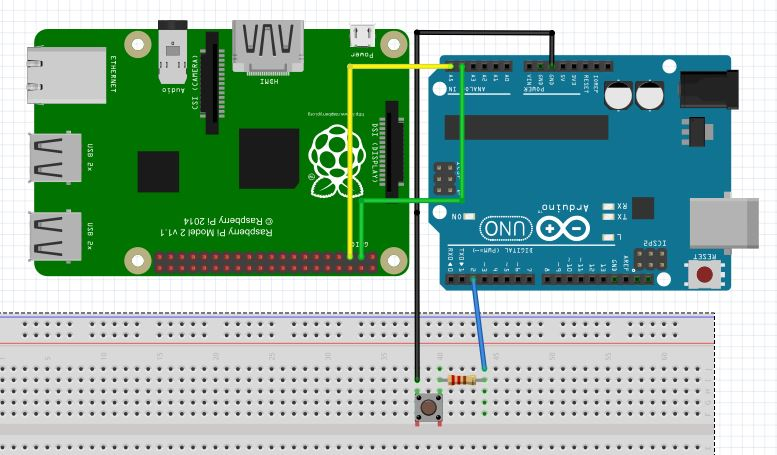
\includegraphics[scale = 0.6]{rpi_with_arduino}
\flushleft
Fig. shows Connection Diagram.
\subsection*{Assembly of harware}
\subsection*{Step 1}
Pin 3(SDA) of Rpi is connected to analog pin A4 of Arduino.
\subsection*{Step 2}
Pin 5(SCL) of Rpi is connected to analog pin A5 of Arduino.
\subsection*{Step 3}
One terminal of resistor is connected to switch and other terminal to digital pin 2 of Arduino.
\subsection*{Step 4}
One terminal of switch is connected to resistor and other terminal to ground.
\section{UART Communication between Firebird V and Raspberry Pi}
\textbf{Connections}  \\
Firebird V is connected with Raspberry Pi using USB cable.\\
\textbf{CODE}\\
Code for Firbird V and Raspberry is available on Github repository.
\section{Software and Code}
\href{https://github.com/eYSIP-2016/eYSIP-Raspberry_Pi_Development_Board}{Github link} for the repository of code

\section{Use and Demo}

\href{https://youtu.be/oxJpwd1q_dY}{Youtube Link} of Accessing GPIO pins of RPi. \\
\href{https://youtu.be/Fn3AqdrCMGo}{Youtube Link} of External Interrupt on Raspberry Pi.\\
\href{https://youtu.be/dhToItyDWhE}{Youtube Link} of I2C Enabling on RPi.\\
\href{https://youtu.be/5fbYMdtAb2E}{Youtube Link} of SPI Enabling on RPi.\\
\href{https://youtu.be/bD0IaSN4_MM}{Youtube Link} of Interfacing Port expander MCP23017 to RPi.\\
\href{https://youtu.be/CWC4LPlKH_k}{Youtube Link} of ADC MCP3008. \\
\href{https://youtu.be/3ISq36l3NLc}{Youtube Link} of Bluetooth communication. \\
\href{https://youtu.be/qROTqvKYI3w}{Youtube Link} of PWM driver PCA9685 IC.   \\


\section{Future Work}
Make a PCB Shield for Raspberry Pi which
will enhance capability of Firebird V robot.\\
Raspberry Pi is an Excellent tool for Dynamic 
and Real time Image Processing. So, by using
Raspberry Pi instead of AtMega 2560 on 
Firebird V we can implement much complex 
themes comprising image processing, as the 
programming in python makes it much easier.

\section{Bug report and Challenges}
Communicating Raspberry Pi with ATMega2560 through UART communication protocol causes a lot of delay which can make the programming task much complicated and the program becomes inefficient.

Any failure or challenges faced during project
\begin{enumerate}
    \item Object Tracking of Firebird V Robot using 3 Sharp IR Sensors using UART communication between Raspberry Pi and ATMega2560.
    \item Courier Service theme of eYRC+ using UART communication between Raspberry Pi and ATMega2560.
    \item Obstacle Avoidance Robot using UART communication between Raspberry Pi and ATMega2560.
\end{enumerate}
These ideas did not work due to delay in communication because of which line following is not at all effective.

\begin{thebibliography}{li}
\bibitem{wavelan97}
Raspbian Jessie OS Installation,
{\em https://www.engadget.com/2012/09/04/raspberry-pi-getting-started-guide-how-to/}
\bibitem{wavelan97}
SPI and I2C communication protocol
{\em www.byteparadigm.com/applications/introduction-to-i2c-and-spi-protocols/}
\bibitem{wavelan97}
I2C configuration
{\em https://learn.adafruit.com/
adafruits-raspberry-pi-lesson-4-gpio-setup/
configuring-i2c}
\bibitem{wavelan97}
Pulse Width Modulation
{\em http://www.electronics-tutorials.ws/blog/
pulse-width-modulation.html}
\bibitem{wavelan97}
Software Interrupt
{\em https://www.techopedia.com/denition/22195/software-interrupt}
\bibitem{wavelan97}
Port expander MCP23017 IC
{\em https://www.mathworks.com/examples/matlab/4547-add-digital-i-o-pins-to-raspberry-pi-hardware-using-mcp23017}
\end{thebibliography}


\end{document}

